\documentclass{beamer}
%\usetheme{PaloAlto}
%\usetheme{Berlin}
\usetheme{Ilmenau}
\usecolortheme{seahorse}

%\usepackage[utf8]{inputenc}
%\usepackage{default}
%\usepackage[italian]{babel}

%\usepackage{titleref}
%\usepackage{zref-titleref}

\usepackage{amsmath}
\usepackage{amssymb}
\usepackage{amsthm}
\usepackage{xfrac}
\usepackage[all]{xy}
\usepackage{mathtools}
\usepackage{graphicx}
%\usepackage{fullpage}
\usepackage{hyperref}
\usepackage[utf8x]{inputenc}
\usepackage[italian]{babel}
\usepackage{mathtools}

%\usepackage{pdftricks}
%\begin{psinputs}
%   \usepackage[pdf]{pstricks}
 %  \usepackage{multido}
%\end{psinputs}

\usepackage{ulem}

\setlength{\parindent}{0in}

\newcounter{counter1}

\theoremstyle{plain}
\newtheorem{myteo}[counter1]{Teorema}
\newtheorem{mylem}[counter1]{Lemma}
\newtheorem{mypro}[counter1]{Proposizione}
\newtheorem{mycor}[counter1]{Corollario}
\newtheorem*{myteo*}{Teorema}
\newtheorem*{mylem*}{Lemma}
\newtheorem*{mypro*}{Proposizione}
\newtheorem*{mycor*}{Corollario}

\theoremstyle{definition}
\newtheorem{mydef}[counter1]{Definizione}
\newtheorem{myes}[counter1]{Esempio}
\newtheorem{myex}[counter1]{Esercizio}
\newtheorem*{mydef*}{Definizione}
\newtheorem*{myes*}{Esempio}
\newtheorem*{myex*}{Esercizio}

\theoremstyle{remark}
\newtheorem{mynot}[counter1]{Nota}
\newtheorem{myoss}[counter1]{Osservazione}
\newtheorem*{mynot*}{Nota}
\newtheorem*{myoss*}{Osservazione}

\newcommand{\obar}[1]{\overline{#1}}
\newcommand{\ubar}[1]{\underline{#1}}

\newcommand{\set}[1]{\left\{#1\right\}}
\newcommand{\pa}[1]{\left(#1\right)}
\newcommand{\ang}[1]{\left<#1\right>}
\newcommand{\bra}[1]{\left[#1\right]}
\newcommand{\abs}[1]{\left|#1\right|}
\newcommand{\norm}[1]{\left\|#1\right\|}

\newcommand{\pfrac}[2]{\pa{\frac{#1}{#2}}}
\newcommand{\bfrac}[2]{\bra{\frac{#1}{#2}}}
\newcommand{\psfrac}[2]{\pa{\sfrac{#1}{#2}}}
\newcommand{\bsfrac}[2]{\bra{\sfrac{#1}{#2}}}

\newcommand{\der}[2]{\frac{\partial #1}{\partial #2}}
\newcommand{\pder}[2]{\pfrac{\partial #1}{\partial #2}}
\newcommand{\sder}[2]{\sfrac{\partial #1}{\partial #2}}
\newcommand{\psder}[2]{\psfrac{\partial #1}{\partial #2}}

\newcommand{\intl}{\int \limits}

\DeclareMathOperator{\de}{d}
\DeclareMathOperator{\id}{Id}
\DeclareMathOperator{\len}{len}

\DeclareMathOperator{\gl}{GL}
\DeclareMathOperator{\aff}{Aff}
\DeclareMathOperator{\isom}{Isom}

\DeclareMathOperator{\im}{Im}



\begin{document}


\title[Oracoli per cammini e distanze]{Cammini minimi su grafi:\\
  oracoli per distanze e cammini}
%\subtitle{}
%\author{Enrico Polesel}
%\institute[Scuola Normale Superiore]{Scuola Normale Superiore}
\date{05 dicembre 2014}

\author[Enrico Polesel]{\begin{tabular}{r@{ }l}
Candidato: &  Enrico Polesel \\ 
Relatore: & Prof. Roberto Grossi
\end{tabular}
}



\begin{frame}[plain]
  \titlepage
\end{frame}

\begin{frame}[plain]
 \frametitle{Indice}
 \tableofcontents
\end{frame}


%\AtBeginSection[]
%{
%  \begin{frame}{\secname}
%    \tableofcontents[currentsection]
%  \end{frame}
%}


\AtBeginSubsection[]
{
  \begin{frame}[plain]{\secname $\rightarrow$ \subsecname}
    \tableofcontents[currentsubsection]
  \end{frame}
}


\section{Grafi e cammini minimi}

\subsection{Grafi e cammini}

\begin{frame}{Definizioni}
  \begin{columns}
    \begin{column}{0.40\textwidth}
      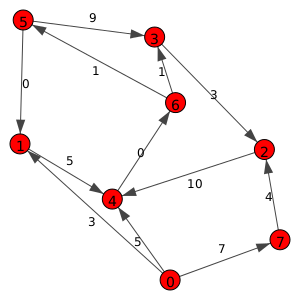
\includegraphics[width=\textwidth]{directgraph}
    \end{column}
    \begin{column}{0.58\textwidth}
      \begin{itemize}
      \item $G = (V,E)$ grafo
      \item $\abs{V} = N$, $\abs{E} = M$
      \item $V$ nodi
      \item $E \subseteq V\times V$ archi
      \item gli archi possono essere orientati
      \item gli archi possono avere un peso $w: E \to \mathbb{R}$ (nel
        nostro caso la lunghezza)
      \end{itemize}
    \end{column}
  \end{columns}
\end{frame}

\begin{frame}{Cammini}
  \begin{columns}
    \begin{column}{0.40\textwidth}
      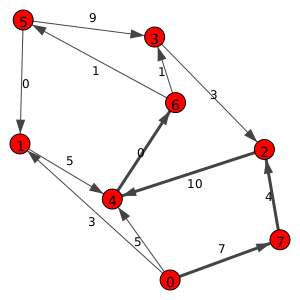
\includegraphics[width=\textwidth]{directpath}
    \end{column}
    \begin{column}{0.58\textwidth}
      \begin{itemize}
      \item Cammino: $p = \pa{ 0,7,2, 4,6}$
      \item Lunghezza: $w(p) = 7+4+10+0 = 21$
      \item $P(u,v) = \set{\text{cammini tra }u\text{ e }v}$
      \item Distanza: $\delta (u,v) = \min \limits _{p\in P(u,v)}
        w(p)$
      \item $\pa{V,\delta}$ \`e una pseudometrica
      \item I cammini minimi sono ``quasi'' aciclici
      \item Sottocammini di cammini minimi sono minimi
      \end{itemize}
    \end{column}
  \end{columns}
\end{frame}

\subsection{Cammini da una sorgente unica}

\begin{frame}{Grafo (aciclico diretto) dei cammini minimi}
  Scegliamo $s\in V$, vogliamo conoscere:
  \begin{itemize}
  \item $\forall v\in V\;\; \delta \pa{s,v}$
  \item $\forall v\in V$ i cammini minimi da $s$ a $v$
  \end{itemize}

  \begin{mypro}
    Se gli archi hanno lunghezza strettamente positiva, il grafo $G_s$
    dei cammini minimi \`e un DAG (grafo aciclico diretto)
  \end{mypro}
  Scegliendo opportunamente un cammino per ogni vertice otteniamo un
  albero.
\end{frame}

\begin{frame}{Archi non pesati: BFS}
    \begin{columns}
    \begin{column}{0.40\textwidth}
      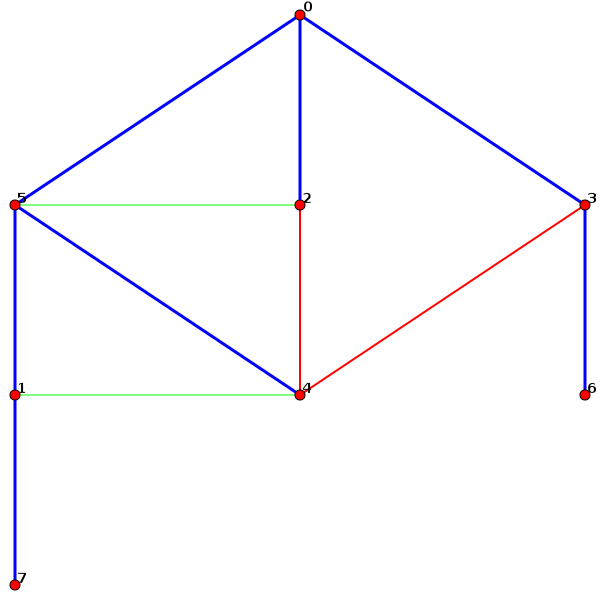
\includegraphics[width=\textwidth]{BFS}
    \end{column}
    \begin{column}{0.58\textwidth}
      Per grafi non pesati (archi di lunghezza unitaria) applicando
      una visita in ampiezza otteniamo distanze e cammini in
      $O\pa{M}$ operazioni.
    \end{column}
  \end{columns}
\end{frame}

\begin{frame}{Archi pesati: algoritmo di Dijkstra}
    \begin{columns}
    \begin{column}{0.40\textwidth}
      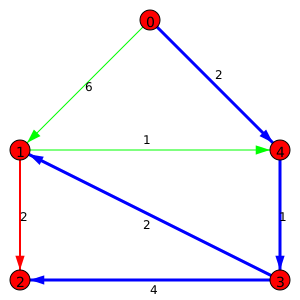
\includegraphics[width=\textwidth]{dijkstraslide} 
    \end{column}
    \begin{column}{0.58\textwidth}
      Per grafi pesati l'algoritmo di Dijkstra costruisce il DAG dei
      cammini minimi in $O\pa{M\log \pa{N}}$ operazioni.
    \end{column}
  \end{columns}  
\end{frame}

\subsection{Cammini tra tutte le coppie}

\begin{frame}{Matrice di adiacenza}
  Numeriamo i vertici: $V = \set{ 0,1,2,..., N-1}$.
  
  \vfill
  Definiamo la matrice $W$ dove
  \begin{itemize}
  \item $W_{i,i} = 0$
  \item $W_{i,j} = w(i,j)$ se $(i,j) \in E$
  \item $W_{i,j} = \infty$ se $(i,j) \not\in E$
  \end{itemize}
 
\end{frame}

\begin{frame}
  Algoritmo
\end{frame}

\begin{frame}
  Ma è un prodotto fra matrici
\end{frame}

\begin{frame}
  Altri risultati
\end{frame}

\begin{frame}{Trovare i cammini minimi}
  Vicini ``buoni''
\end{frame}


\subsection{$k$ cammini pi\`u brevi}

\begin{frame}
  Problema e risultati
\end{frame}


\section{Oracoli per distanze}

\subsection{Oracoli approssimati}

\begin{frame}{Graph spanner}
  
\end{frame}

\begin{frame}{Risultati}
  
\end{frame}

\subsection{Oracoli esatti}

\begin{frame}{Limiti teorici}
  
\end{frame}

\begin{frame}{Albero etichettato}
  
\end{frame}

\begin{frame}{Somme prefisse}
  
\end{frame}


\section{Oracoli per cammini}

\subsection{Algoritmi facili}

\begin{frame}{Un oracolo}
  
\end{frame}

\begin{frame}{Un non oracolo}
  
\end{frame}

\subsection{Grafi planari}

\begin{frame}{Separation theorem}
  
\end{frame}

\begin{frame}{Un oracolo}
  
\end{frame}

\subsection{Miglioramenti dell'oracolo facile}

\begin{frame}{Miglioramento}
  
\end{frame}

\begin{frame}{Struttura dei cammini}
  
\end{frame}

\begin{frame}{Caso pessimo}
  
\end{frame}

\subsection{Costruzione di un caso difficile}

\begin{frame}{Grafo bipartito}
  
\end{frame}

\begin{frame}{Intersezione di insiemi}
  
\end{frame}


\end{document}







